\documentclass[11pt]{article}
\usepackage[margin=0.7in]{geometry}
\usepackage{amsmath,amssymb}
\usepackage{enumitem}
\usepackage{tikz}
\usepackage{pgfplots}
\pgfplotsset{compat=1.18}
\usepackage{fancyhdr}
\usepackage{parskip}
\setlist[enumerate]{leftmargin=*, itemsep=6pt}
\pagestyle{fancy}
\fancyhf{}
\fancyfoot[L]{\small\textit{en}Vision\textsuperscript{\textregistered} Algebra 2}
\fancyfoot[C]{\small 5-6 Lesson Quiz, short form}
\fancyfoot[R]{\small\thepage}
\renewcommand{\headrulewidth}{0pt}
\newcommand{\choice}[1]{\tikz[baseline=-0.6ex]\node[draw, circle, inner sep=0.6pt, minimum size=3.3mm, font=\scriptsize\bfseries] {#1};\;}
\newcommand{\checkbox}{$\square$\;}
\pgfplotsset{quizgrid/.style={
  axis lines=middle, grid=both, grid style={gray!45},
  ticklabel style={font=\scriptsize, fill=white, inner sep=1pt},
  xlabel={$x$}, ylabel={$y$}, axis line style={thick}, clip=true}}

\begin{document}

\noindent\textbf{Name}\; \rule{6cm}{0.4pt} \hfill Period \rule{1.2cm}{0.4pt} \quad Date \rule{2.2cm}{0.4pt}

\vspace{4pt}\noindent\rule{\textwidth}{0.6pt}

\vspace{2pt}\noindent{\LARGE\textbf{5-6 \; Lesson Quiz: Inverse Relations and Functions}} \hfill {\small short form}

\vspace{4pt}\noindent\rule{\textwidth}{0.6pt}

{\small Question numbers match the Savvas Lesson Quiz (questions 1 and 4 are not on this form).}

\vspace{4pt}
\begin{minipage}[t]{0.50\textwidth}
\textbf{2.} Sketch the graph of $f$ and the inverse of $f$, if $f(x)=\tfrac12x+3$.

\vspace{8pt}
Show your work: switch $x$ and $y$ and solve for $y$ (or swap the coordinates of two points of $f$).

\vspace{10pt}
$y=\tfrac12x+3$ \;$\longrightarrow$\; $x=\rule{3cm}{0.4pt}$

\vspace{14pt}
\rule{\linewidth}{0.4pt}

\vspace{14pt}
$f^{-1}(x)=\rule{3.4cm}{0.4pt}$
\end{minipage}\hfill
\begin{minipage}[t]{0.46\textwidth}
\vspace{-6pt}
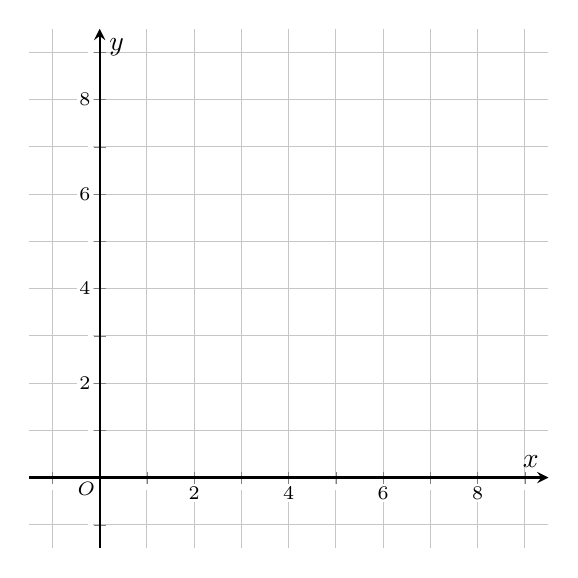
\begin{tikzpicture}
% TE: unit grid x, y from -1 to 9, labels 2,4,6,8 and origin O; window padded 0.5.
\begin{axis}[quizgrid, xmin=-1.5, xmax=9.5, ymin=-1.5, ymax=9.5,
  xtick={-1,...,9}, ytick={-1,...,9}, xticklabels={,,,2,,4,,6,,8,}, yticklabels={,,,2,,4,,6,,8,},
  x=0.6cm, y=0.6cm]
\node[font=\scriptsize, anchor=north east, inner sep=1.5pt] at (axis cs:0,0) {$O$};
\end{axis}
\end{tikzpicture}
\end{minipage}

\vspace{10pt}\noindent\rule{\textwidth}{0.4pt}

\vspace{6pt}
\textbf{3.} Let $f(x)=x^2-2x+1$. Find the inverse function of $f$ by identifying an appropriate restriction of its domain.

\vspace{4pt}
\begin{itemize}[leftmargin=1.2em, itemsep=5pt]
\item[] \choice{A} The inverse is $f^{-1}(x)=\sqrt{x+1}$ if the domain of $f$ is restricted to $x\geq-1$.
\item[] \choice{B} The inverse is $f^{-1}(x)=\sqrt{x}+1$ if the domain of $f$ is restricted to $x\geq1$.
\item[] \choice{C} The inverse is $f^{-1}(x)=\sqrt{x}-1$ if the domain of $f$ is restricted to $x\geq0$.
\item[] \choice{D} The function does not have an inverse.
\end{itemize}

\vspace{6pt}
Show your work. Write $f$ as a square, name the vertex, then switch $x$ and $y$:

\vspace{14pt}\rule{\linewidth}{0.4pt}

\vspace{14pt}\rule{\linewidth}{0.4pt}

\vspace{6pt}\noindent\rule{\textwidth}{0.4pt}

\vspace{6pt}
\textbf{5.} Let $f(x)=2x+4$ and $g(x)=\tfrac12x-2$. Complete the sentence. Check \textbf{one} box.

\vspace{4pt}
The function $g(x)=\tfrac12x-2$ \rule{4cm}{0.4pt} $f(x)=2x+4$.

\vspace{2pt}
\checkbox is the inverse of \qquad \checkbox is equivalent to \qquad \checkbox is the opposite of \qquad \checkbox has the same intercepts as

\vfill
\noindent\textbf{Scoring:} Question 2 and Question 3 are 10 points each. Question 5 is a bonus of 5 points. Total out of 20.

\newpage
\noindent{\LARGE\textbf{5-6 Lesson Quiz, short form: answer key}}

\vspace{4pt}\noindent\rule{\textwidth}{0.6pt}

\begin{enumerate}
\item[\textbf{2.}] \textbf{Graph of $f$ and $f^{-1}$.} $f$ is the line through $(0,3)$ with slope $\tfrac12$ (also $(2,4)$, $(6,6)$). Switch and solve: $x=\tfrac12y+3$, $2(x-3)=y$, so $f^{-1}(x)=2x-6$: the line through $(3,0)$ with slope $2$ (also $(4,2)$, $(6,6)$). The two lines are reflections across $y=x$ (for the teacher: they cross at $(6,6)$ on $y=x$; students are not asked for it). TE key: graph shown (two lines, shallow $f$ with $y$-intercept 3, steep inverse with $x$-intercept 3, crossing at $(6,6)$). Savvas quiz item 2, DOK 2, skill F65. \textbf{10 points:} 4 for the graph of $f$, 4 for the graph of the inverse, 2 for the work shown (the equation $f^{-1}(x)=2x-6$, or two points of $f$ with their coordinates swapped).
\item[\textbf{3.}] \textbf{B.} $f(x)=x^2-2x+1=(x-1)^2$, vertex $(1,0)$. Restrict to $x\geq1$; then $x=(y-1)^2$, $\sqrt{x}=y-1$, $f^{-1}(x)=\sqrt{x}+1$, $x\geq0$. Distractor A is the inverse of $x^2-1$ and C of $(x+1)^2$: each starts from the wrong vertex. Savvas quiz item 3, DOK 2, skill F65. \textbf{10 points:} 6 for B, 4 for the work (the square $(x-1)^2$ or the vertex, and the switch).
\item[\textbf{5.}] \textbf{is the inverse of.} $x=2y+4$ gives $y=\tfrac12x-2=g(x)$. Check: $f(g(x))=2(\tfrac12x-2)+4=x$. Savvas quiz item 5, DOK 2, skill F65. \textbf{Bonus 5:} the inverse box and no other.
\end{enumerate}

\textbf{Items left off this form} (available for a retake or Form B): Savvas item 1, missing values in the table of the inverse (answer $a=-1$, $b=1$, $c=3$, $d=-2$; DOK 1, F65; the packet's ``switch the columns'' table rehearses it); Savvas item 4, inverse of $f(x)=\tfrac12\sqrt[3]{x-3}+5$ in the form $f^{-1}(x)=\rule{0.5cm}{0.4pt}+\rule{0.5cm}{0.4pt}(x-\rule{0.5cm}{0.4pt})^3$ (answer $3$; $8$; $5$, that is $f^{-1}(x)=3+8(x-5)^3$; DOK 2, F65; taught by Example 4, cut from the fast packet).

\textbf{IXL replacement:} SmartScore 70 or above on ZRQ, K2W and 9KT replaces this quiz with 20/20.

\end{document}
